\documentclass[12pt]{article}

\usepackage[dvips,letterpaper,margin=0.75in,bottom=0.75in]{geometry}
\usepackage{cite}
\usepackage{slashed}
\usepackage{graphicx}
\usepackage{amsmath}

\usepackage[american,fulldiode]{circuitikz}
\usetikzlibrary{calc}

\begin{document}
\ctikzset{bipoles/thickness=2}

\title{Lab 2:  Operational Amplifiers}

\maketitle

\section{Pre-lab Calculations}
\noindent



1) Calculate the gain for all four circuits in Fig.~\ref{fig:common}. \\

\section{Introduction}

Operational Amplifiers?  They should call them fun amplifiers.  Because, man, are they fun.  Get ready for some fun!

We'll be building a number of op-amp circuits using the classic LM741 operation amplifier of Fig~\ref{fig:lm741layout}.  We'll use an op-amp current source and differential amplifier to build a do-it-yourself transistor diode curve tracer and use it to measure the diode curve of a 2N3904 NPN transistor (see Fig~\ref{fig:2n3904layout}).

%DEBUG:  \pgfcircversion{}

\begin{figure}[htbp]
\begin{center}
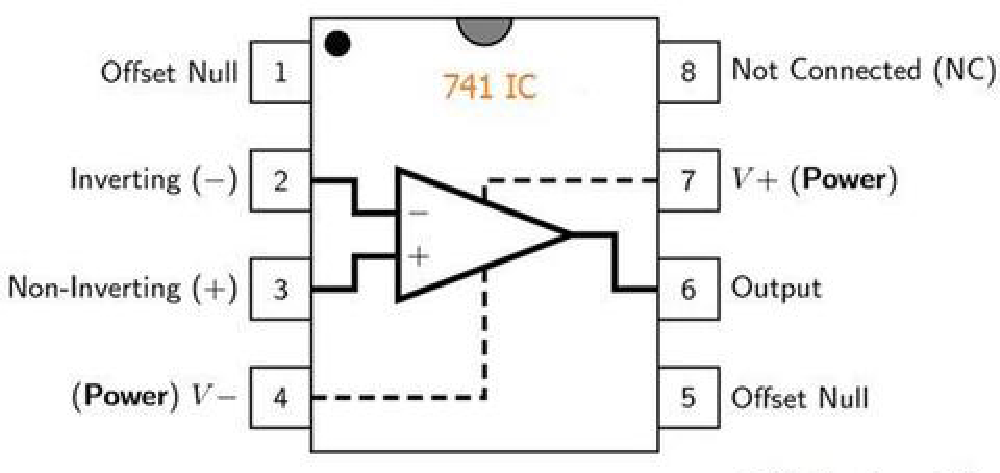
\includegraphics[height=0.15\textheight]{figs/lm741.pdf} 
\end{center}
\caption{The LM741 8-DIP layout.}
\label{fig:lm741layout}
\end{figure}

\begin{figure}[htbp]
\begin{center}
\begin{tabular}{c@{\hskip 2cm}c}
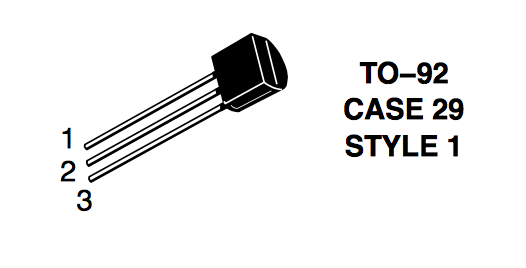
\includegraphics[height=0.10\textheight]{figs/case3904.png} &
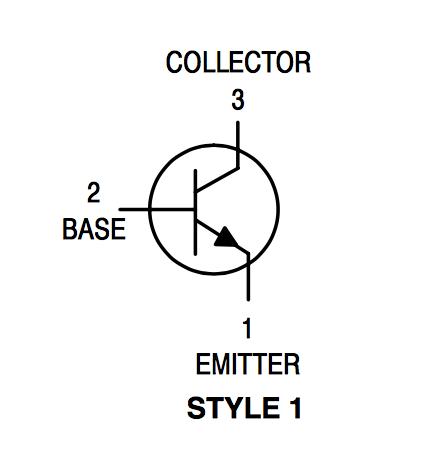
\includegraphics[height=0.18\textheight]{figs/pinout3904.png} \\
\end{tabular}
\end{center}
\caption{The TO-92 Style 1 package used for some discrete transistors,
including the 2N3904 (NPN) and 2N3906 (PNP) transistors used throughout this lab.  Note that
not all transistors use the same pinout, even if they are in the TO-92
package.}
\label{fig:2n3904layout}
\end{figure}

\section{Common Op-Amp Circuits}

\begin{figure}[htbp]
\begin{center}
\begin{tabular}{c@{\hskip 0.25in}c}
\begin{circuitikz}[]
\draw
(0,0) node[op amp](opamp){}
(opamp.+) to[short,-o] ++(-.5,0) node[left]{$v_{\rm in}$}
(opamp.-) to[short] ++ (0,+0.75)  to[short] ++(2.0,0) -| (opamp.out)
(opamp.out) to[short,*-o] ++ (0.5,0) node[right]{$v_{\rm out}$}
;
\end{circuitikz} &
\begin{circuitikz}
\draw
(0,0) node[op amp](opamp){} 
(opamp.+) to[short,-o] ++(-.5,0) node[left]{$v_{\rm in}$}
(opamp.-) to[short] ++ (0,1.0) coordinate(X) to[R,l_=$R_2$,bipoles/length=1cm] ++(2.25,0) -| (opamp.out)
(opamp.-) to[R,l_=$R_1$,bipoles/length=1cm] ++(-2,0) node[ground,yscale=1.5]{}
(opamp.out) to[short,*-o] ++ (0.5,0) node[right]{$v_{\rm out}$}
;
\end{circuitikz} \\
(a) & (b) \\ 
&\\
\begin{circuitikz}[]
\draw
(0,0) node[op amp](opamp){} 
(opamp.-) to[R,l_=$R_1$,*-o,,bipoles/length=1cm] ++(-1.5,0) node[left]{$v_{\rm in}$}
(opamp.+) to[short] ++(0,-0.5) node[ground,yscale=1.5]{}
(opamp.-) to[short] ++ (0,1.0) to[R,l_=$R_2$,bipoles/length=1cm] ++(2.25,0) -| (opamp.out)
(opamp.out) to[short,*-o] ++ (0.5,0) node[right]{$v_{\rm out}$}
;
\end{circuitikz} &
\begin{circuitikz}[]
\draw
(0,0) node[op amp](opamp){} 
(opamp.-) to[R,l=$R_1$,*-o,,bipoles/length=1cm] ++(-1.5,0) node[left]{$v_{\rm 2}$}
(opamp.+) to[short] ++(0,-0.5) node[ground,yscale=1.5]{}
(opamp.-) to[short] ++ (0,1.0) coordinate(X) to[R,l_=$R_2$,bipoles/length=1cm] ++(2.25,0) -| (opamp.out)
(X) to[R,l=$R_3$,*-o,bipoles/length=1cm] ++(-1.5,0) node[left]{$v_{\rm 1}$}
(opamp.out) to[short,*-o] ++ (0.5,0) node[right]{$v_{\rm out}$}
;
\end{circuitikz} \\
(c) & (d) \\
\end{tabular}
\caption{Common Op-Amp circuits: (a) Follower, (b) Non-Inverting Amplifier, (c) Inverting Amplifier, and (d) Adder.}
\label{fig:common}
\end{center}
\end{figure}


\noindent 
In this section you will build the four common op-amp circuits shown in Fig.~\ref{fig:common} using a single LM741 op-amp.  In all four circuits use $R_1 = 22~\rm k\Omega$, $R_2 = 220~\rm k\Omega$, $R_3 = 22~\rm k\Omega$ wherever they appear.  The power supply connections are not shown, but should be provided using both channels of your bench-top DC supply as $V_+=+10~\rm V$
and $V_-=-10~\rm V$.  

Start with the follower circuit (Fig.~\ref{fig:common}a) and confirm the gain using an input signal provided by your function generator with an AC signal with $V_{\rm RMS} = 200~\rm mV$ at a frequency of $1~\rm kHz$.  Whenever I use an op amp, I almost always first build a follower circuit.  It's super easy to do, since it needs no resistors, and it confirms that your power supplies, inputs, and outputs, are all connected in the right place before moving on to a more complicated circuit.

Next build the non-inverting amplifier by adding resistors $R_2$ and $R_1$ as in Fig.~\ref{fig:common}b, and confirm the gain.  Then build the inverting amplifier of Fig.~\ref{fig:common}c by interchanging the connection points for $v_{\rm in}$ and ground and confirm the gain.   

For the adder, or summing amplifier, in Fig.~\ref{fig:common}d add resistor $R_3$ and provide an additional input using the second channel of your function generator with an AC signal with $V_{\rm RMS} = 200~\rm mV$ at a frequency of $5~\rm kHz$.  Does the resulting output make sense?

\section{Log Amplifier}

\begin{figure}[htbp]
\begin{center}
\begin{circuitikz}
\draw
(0,0) node[op amp](opamp){} 
(opamp.-) to[R,bipoles/length=1cm,l_=$R_1$,*-*] ++(-1.5,0) node[left]{$v_{\rm in}$}
(opamp.+) to[short] ++(0,-0.5) node[ground,yscale=1.5]{}
(opamp.-) to[short] ++ (0,1.0) to[D,l_=$D$,bipoles/length=0.6cm] ++(2.25,0) -| (opamp.out)
(opamp.out) to[short,*-o] ++ (0.5,0) node[right]{$v_{\rm out}$}
;
\end{circuitikz} 
\caption{Log amplifier}
\label{fig:logamp}
\end{center}
\end{figure}

\noindent
The nifty circuit in Fig.~\ref{fig:logamp} provides logarithmic output:
\begin{displaymath}
v_{\rm out} = - n v_T \log\left(\frac{v_{\rm in}}{I_o R_1} \right)
\end{displaymath}
Build it from your adder by removing the second input resistor ($R_3$) and replacing the feedback resistor ($R_2$) with a 1N4001 diode.
You cannot take the log of a negative number, so drive the circuit with an offset AC signal with a minimum of $0~\rm V$ and a maximum of $2~\rm V$.  Measure $v_{\rm in}$ on channel 1 of your scope with DC coupling.  Measure $v_{\rm out}$ on channel 2 of your scope with DC coupling and invert set to ``On".  
View the output in XY mode and confirm the logarithmic shape.

\section{Differential Follower}

\begin{figure}[htbp]
\begin{center}
\begin{circuitikz}
\draw
(0,0) node[op amp](opamp){} 
(opamp.-) to[R,bipoles/length=1cm,l_=$R_1$,*-o] ++(-1.5,0) node[left]{$v_{\rm in}^-$}
(opamp.+) to[R,bipoles/length=1cm,l=$R_1$,*-o] ++(-1.5,0) node[left]{$v_{\rm in}^+$}
(opamp.+) to[R,bipoles/length=1cm,l=$R_2$] ++(0,-2.0) node[ground,yscale=1.5]{}
(opamp.-) to[short] ++ (0,1.0)  to[R,bipoles/length=1cm,l=$R_2$] ++(2.25,0) -| (opamp.out)
(opamp.out) to[short,*-o] ++ (0.5,0) node[right]{$v_{\rm out}$}
;
\end{circuitikz} 
\caption{A differential amplifer.}
\label{fig:diffamp}
\end{center}
\end{figure}

\noindent
The circuit in Fig.~\ref{fig:diffamp} is a differential amplifier which reduces to a differential follower:
\begin{displaymath}
v_{\rm out} = v_{\rm in}^+ - v_{\rm in}^- 
\end{displaymath}
when $R_1 = R_2$.  Build the circuit using $R_1 = R_2 = 22~\rm k\Omega$ and confirm it's operation using two input signals from your function generator.  {\bf Once you have this circuit working, save it for use later on in the lab!}

\section{Current Source}

\begin{figure}[htbp]
\begin{center}
\begin{tabular}{c@{\hskip 0.25in}c}
\begin{circuitikz}
\draw
(0,0) node[op amp](opamp){} 
++(2,0) node[pnp](pnp){}
(opamp.out) to[short] (pnp.B)
(pnp.E) to[short,-*] ++(0,0.5) coordinate(X) to[R,bipoles/length=1cm,l=$R_3$,-*] ++(0,1.0) coordinate(A) to[short,-o] ++(0,0.5)node[right]{$V_+$}
(X) -| (opamp.-)
(pnp.C) node[right]{$P_{\rm src}$} to[R,bipoles/length=1cm,l=$R_{\rm L}$,o-] ++(0,-1.5) coordinate(B) node[ground,yscale=1.5]{} 
(opamp.+) to[short] ++(-0.5,0) coordinate(X) to[short] ++(0,1.75) to[R,bipoles/length=1cm,l_=$R_2$] ++(0,1.0) |- (A)
(X) to[short] ++(0,-0.75) to[R,bipoles/length=1cm,l=$R_1$] ++(0,-0.5) |- (B)
;
\end{circuitikz} &
\begin{circuitikz}
\draw
(0,0) node[left]{$V_+$} to[I,l=$I_{\rm src}$,bipoles/length=1.25cm,o-o] ++ (0,-2)
node[right]{$P_{\rm src}$} to[R,bipoles/length=1cm,l=$R_{\rm L}$,o-] ++(0,-1.5) node[ground,yscale=1.5]{} 
;
\end{circuitikz} \\
(a) & (b) \\
\end{tabular}
\caption{A current source (a) as build, and (b) modeled as an ideal current source.}
\label{fig:current}
\end{center}
\end{figure}

Use a {\bf second} LM741 op-amp and a 2N3906 PNP transistor to build the current source shown in Fig.~\ref{fig:current}.  Use $R_2 = R_3 = 10~\rm k\Omega$ and $R_1 = 47~\rm k\Omega$.  Test using $R_L = R_1$ and $R_L = R_1/10$, and $R_L=0$.  You should see a nearly constant current through the resistor $R_3$.  {\bf Once you have this circuit working, save it for use later on in the lab!}

Take a moment to marvel at the power of negative feedback.  The op-amp knows absolutely nothing about diode drops and transistor transconductance.  And yet, simply because of feedback, it manages to hold the voltage of the transistor base at exactly the right point to provide the desired current.  Feedback belongs alongside resonance on our list of humanity's greatest tricks!

\section{Transistor Curve Tracer}
\begin{figure}[htbp]
\begin{center}
\begin{circuitikz}
\draw
(0,0) node[npn](npn1){} 
(npn1.C) to[R,bipoles/length=0.8cm,l=$R$] ++(0,+1.5) coordinate(A)
(npn1.C) to[short,*-o] ++(0.5,0) node[right]{$v_1 \to v_{\rm in}^-$}
(A) to[short,*-o] ++(0.5,0) node[right]{$v_2 \to v_{\rm in}^+$}
(npn1.E) node[ground,yscale=1.5]{}
(npn1.B) ++(-2.0,0) node[left]{$V_+$} to[I,bipoles/length=1.25cm,l_=$I_{\rm src}$,o-o] (npn1.B)
++(-0.15,0) node[below]{$P_{\rm src}$};
\path let \p1 = (npn1.E) in coordinate(B) at (-4,\y1);
\draw
(A) to[short] ++(-4,0) to[sinusoidal voltage source,bipoles/length=1.25cm,l=$\tilde{V}$] ++(0,-1.5) 
to[short] (B) node[ground,yscale=1.5]{}
;
\end{circuitikz} 
\caption{A DIY transistor curve tracer.}
\label{fig:tracer}
\end{center}
\end{figure}

\noindent
In this section, you will build a transistor curve tracer to observe transistor curves using your oscilloscope.

Connect the emitter of an 2N3904 NPN transistor, the device under test (DUT), to ground and drive the base with your current source from the previous section.  Confirm that a diode drop is found across the $B$-$E$ junction.  Next, drive the collector of the DUT through a $100~\rm \Omega$ resistor with your function generator set to provide an offset AC signal with minimum $0~\rm V$ and maximum $5~\rm V$.

The transistor curve for $I_C$ versus $V_CE$ at fixed $I_B$ will result if you monitor $v_2-v_1$
(proportional to $I_C$) versus $v_1$ ($V_CE$)on your oscilloscope.  Connect the ground shield clips from both scope probes to ground, and connect $v_1$ to channel 1 on your scope.  The differential follower
from the preceding section is needed to provide the voltage $v_2-v_1$ referenced to ground, suitable for viewing using the single remaing oscilloscope probe.  Connect $v_1$ to the inverting input of your differential amplifier, and $v_2$ to the non-inverting input.  Then connect the output of the differential follower to the tip of the channel 2 scope probe.  With the scope in $X$-$Y$ mode, a transistor $I_C$ versus $V_{\rm CE}$ should result.

By monitoring the voltage across $R_3$ in your current source (Fig.~\ref{fig:current}) you can monitor the current into the base of the transistor.  Adjusting the DC supply voltage will (via the voltage divider used to bias the current source) will adjust the fixed current sent to base of the DUT, resulting in a different curve in $V_{\rm CE}$ versus $I_C$.

Adjust the DC supply voltage to provide $50~\rm \mu A$ of current to the base.  Then adjust the DC supply to provide $100~\rm \mu A$ of current to the base.  You should observe the plateau of the transistor curve to increase by a factor of two.

If time permits, try to estimate both $\beta$ and the early voltage of this transistor using the observed curves.

\section{Lab Report}

Your report should include all of your measurements and comparisons with your calculations.
 
\end{document}
